\section{Zielsetzung}
Im vorliegenden Versuch soll das temperaturabhängige Verhalten von Dipolen in Ionenkristallen untersucht werden.
Hierzu sollen die Aktivierungsenergie $W$ und die charakteristische Relaxationszeit $\tau_{0}$ einer Probe bestimmt werden.

\section{Theorie}
Werden zweiatomige Kationen in ein einatomiges Ionenkristallgitter
eingebaut entstehen aufgrund der Ladungsneutralität, wie in Abblidung \ref{fig:aufbau} dargestellt, Kation-Leerstellen.
Die Verbindungslinie zwischen dem eingebauten Kation und der Leerstelle gibt
die Richtung des Dipols an, welcher sich zwischen diesen beiden
Punkten ausbildet.
Eine Richtungsänderung dieses Dipols kann aufgrund der Gittereigenschaften
nur durch Leerstellendiffusion und somit nur in diskreten Werten erfolgen.
Um diesen Prozess zu bewirken muss Energie in Form von Wärme in das System gebracht werden, bis
eine bestimmte Aktivierungsenergie $W$ erreicht wird.
Die Dipole, die aufgrund ihrer thermischen Bewegung dazu in der Lage sind,
diese Schwellenenergie aufzunehmen, sind nach der Boltzmannstatistik verteilt.
Hierzu proportional ist die mittlere Zeit zwischen zwei Umorientierungen des Dipols, auch Relaxationszeit genannt.
\begin{equation}
\tau (T)=\tau_{0}\exp(W/kT)
\label{eqn:rel}
\end{equation}
 Hierbei ist $k$ die Boltzmannkonstante, $T$ die Temperatur und $\tau_{0}$ die
 charakteristische Relaxationszeit für die $\tau_{0}=\tau(\infty)$ gilt.\\
 Mittels eines elektrischen Feldes $E$ lässt sich aufgrund der thermischen
 Bewegung der Gitterbausteine nur ein Bruchteil $y$ der Dipolgesamtheit aus der statistischen Verteilung
 über alle Raumwinkel hin zum E-Feld ausrichten. Der Bruchteil $y$ wird mit der
 Langevin-Funktion $L(x)$ beschrieben, wobei $x=\frac{pE}{kT}$ mit dem Dipolmoment $p$ ist.
 Da $x<\!<1$ wegen $pE<\!<kT$ lässt sich $y$ aufgrund der Eigenschaften der Langevin-Funktion als
 \begin{equation}
 y=\frac{pE}{3kT}
 \end{equation}
 schreiben.
 \begin{figure}[H]
 \centering
 \begin{subfigure}{0.49\textwidth}
 \centering
 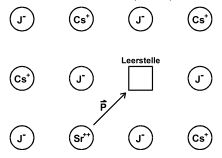
\includegraphics[width=6.5cm]{kristall.JPG}
 \caption{Dipol am Beispiel eines CsJ-Gitters mit Sr$^{2+}$-Kation \cite{V48}}
 \label{fig:aufbau}
 \end{subfigure}
 \begin{subfigure}{0.49\textwidth}
 \centering
 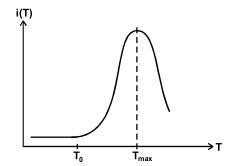
\includegraphics[width=6.5cm]{verlauf.JPG}
 \caption{Erwarteter Verlauf der Stromdichte gegenüber der Temperatur \cite{V48}}
 \label{fig:kurv}
 \end{subfigure}
 \caption{Einfache Darstellung eines Dipols und der Verlauf der zumessenden Stromdichte}
 \end{figure}
 Bedingung für die Gültigkeit dieser Formel ist, dass die Zeit $t$ in der das E-Feld
 die Dipole ausrichtet groß gegenüber der Relaxationszeit $\tau(T)$ ist.
Durch schnelles Abkühlen dieser Verteilung der Ausrichtung des Bruchteils $y$ der Dipole entlang des E-Feldes, gelingt es, aufgrund des exponentiellen Anstiegs
der Relaxationszeit mit sinkender Temperatur, die Dipolausrichtungen einzufrieren.
Durch das Kurzschließen und damit einhergehende Entladen der
%das E-Feld erzeugenden
Kondesatorplatten wird sichergestellt, dass keine freien beweglichen Elektronen den Depolarisationsstrom beeinflussen.
Dieser entsteht durch das Aufheizen der Probe mit einer konstanten Heizrate $b=\frac{dT}{dt}$ und dem damit verbundenen Relaxieren der Dipole zurück in die räumliche Winkelverteilung.
Die Depolarisationsstromdichte $j(t)$ ergibt sich nach
\begin{equation}
  j(T) = y(T_\text{P}) p \frac{dN}{dt},
\label{eqn:strom}
\end{equation}
 mit $T_{P}$ als Polarisationstemperatur und $\frac{dN}{dt}$ als Zahl der pro Zeit und Volumeneinheit relaxierenden Dipole.
 Der erwartete Verlauf der Depolarisationsstromdichte gegen die Temperatur ist in Abbildung \ref{fig:kurv} dargestellt.
Dieser Verlauf ergibt sich aufgrund der schnellen Abnahme der Relaxationszeit bis zu einem Maximum.
Danach nimmt die Depolarisationsstromdichte wieder ab, da die Zahl der noch nicht relaxierten Dipole abnimmt und somit im gleichen Temperaturintervall weniger Dipole relaxieren können.
Der Faktor $\frac{dN}{dt}$ ist mit dem Proportionalitätsfaktor $\frac{1}{\tau}$ proportional zur Zahl
der noch pro Volumeneinheit orientierten Dipole.
\begin{equation}
\frac{dN}{dt}=\frac{N}{\tau}
\label{eqn:dif1}
\end{equation}
Die Lösung dieser Differentialgleichung ist
\begin{equation}
N=N_{\text{P}}\exp{\left(-\frac{1}{b}\int_{T_{0}}^{T} \frac{dT'}{\tau(T')}\right)}
\label{eqn:N}
\end{equation}
$N_{\text{P}}$ ist dabei die Dipolzahl zu Beginn des Aufheizens also bei der Temperatur $T_{0}$.
Das lässt sich nun mittel Gleichung \ref{eqn:dif1} in Formel \ref{eqn:strom} einsetzen und $\tau(T)$ durch Formel \ref{eqn:rel} ersetzen.
So erhält man für die Depolarisationsstromdichte
\begin{equation}
j(T)=\frac{p^{2}EN_{\text{P}}}{3kT_{\text{P}}\tau_{0}} \exp{\left(-\frac{1}{b\tau_{0}}\int_{T_{0}}^{T}\exp{-\left(\frac{W}{kT'}\right)dT'}\right)}\exp{\left(-\frac{W}{kT}\right)}  .
\label{strom02}
\end{equation}
Um nun die gesuchte Potentialschwelle $W$ zu erhalten gibt es zwei Methoden.
Für eine möglichst genaue Bestimmung der Potentialschwelle $W$ wird Methode~1 angewandt, bei der
die Schwellenenergie aus dem gesammten Kurvenverlauf bestimmt wird.
Hierzu wird für die Polarisation $P$ eine Differentialgleichung analog
zu Gleichung \ref{eqn:dif1} aufgestellt.
\begin{equation}
  \frac{dP}{dt}=\frac{P(t)}{\tau(T(t))}
\end{equation}
Durch die Integration des durch die Polarisation erzeugten Stromes $i(t)$
ergibt sich nun einen Ausdruck für
\begin{equation}
  \tau(T(t))=\frac{\int_{t(T)}^{\infty} i(t) dt}{i(t(T))} .
  \label{eqn:taum2}
\end{equation}
Da $t$ und $T$ über eine lineare Funktion zusammenhängen, lässt sich Gleichung \ref{eqn:taum2} auch als
\begin{equation}
  \tau(T)=\frac{\int_{T}^{\infty}i(T')dT'}{bi(T)}
\end{equation}
schreiben. Mit Formel \ref{eqn:rel} lässt sich nun ein Zusammenhang mit
der Aktivierungsenergie $W$ herstellen.
\begin{equation}
  \frac{W}{kT}=\frac{\int_{T}^{\infty}i(T')dT'}{bi(T)\tau_{0}}
  \label{eqn:strom2}
\end{equation}
Somit lässt sich nun $W$ bestimmen indem
\begin{equation}
  \ln \frac{\int_{T}^{T*}i(T')dT'}{i(T)}
  \label{eqn:11}
\end{equation}
gegen $\frac{1}{T}$ aufgetragen wird. $T^*$ ist dabei eine beliebige Temperatur
bei der $i(T) \approx 0$ gilt.
  $\tau_{0}$ lässt sich bestimmen, indem zunächst Gleichung \ref{eqn:stmet1} nach $T$ differenziert wird und
 gleich 0 gesetzt wird.
 \begin{equation}
   \frac{\text{d}}{\text{d}T} \left( \frac{p^{2}EN_{\text{P}}}{3kT_{\text{P}}\tau_{0}} \exp{\left(-\frac{1}{b\tau_{0}}\int_{T_{0}}^{T}\exp{-\left(\frac{W}{kT'}\right)dT'}\right)}\exp{\left(-\frac{W}{kT}\right)} \right)= 0
 \end{equation}
Nun wird $T=T_{\text{max}}$ gesetzt und der Vorfaktor durch Dividieren eliminiert. So erhält man
\begin{equation}
  0=\frac{W}{kT_{\text{max}}^{2}}-\frac{1}{b\tau_{0}}\exp{\left(-\frac{W}{kT_\text{max}^2}\right)}
\end{equation}
 Daraus
 lässt sich $\tau_{0}$ also als
 \begin{equation}
   \tau_{0}=\frac{kT_\text{max}^{2}}{Wb} \exp{\left(-\frac{W}{kT_\text{max}^2}\right)}
   \label{eqn:tau}
 \end{equation}
 bestimmen.
 Eine weitere, mit weniger Rechenaufwand verbundene Möglichkeit die Potentialschwelle $W$ zu bestimmen, ist
Methode~2. Hierbei lässt sich im Anfangsbereich der Kurve der Depolarisationsstrom wegen
 \begin{equation}
 \int_{T_{0}}^{T'} \exp{\left(-\frac{W}{kT}\right)}dT' \approx 0
 \label{eqn:7}
 \end{equation}
 als
 \begin{equation}
 j(T) \approx \frac{p^{2}E N_{\text{P}}}{3k T_{\text{P}}\tau_{0}} \exp{\left(-\frac{W}{kT}\right)}
 \label{eqn:stmet1}
 \end{equation}
 nähern.
 Für den Temperaturbereich indem diese Näherung gültig ist,
 lässt sich W aus der Steigung der Ausgleichsgeraden die durch ein Diagramm gelegt wird, in dem
 $\ln(j)$ gegen $\frac{1}{T}$ augetragen ist, berechnen.\\
